
\chapter{Related work}\label{sec:rel}
This thesis is centred around the study of the \emph{implementability 
problem} for \emph{global types} and MSC-based formal models.  
In this chapter, I review related works addressing this problem, 
both within the same formal framework and in comparable models.  

In particular, this thesis forms part of a broader line of research 
originating from~\cite{di2023partial} and later expanded in 
\cite{di2025realisability}, which aims to develop a general framework 
for communication models. I first present and discuss the results of 
these works, positioning my own contributions in relation to them.  

Subsequently, I analyse recent results by 
Stutz~et~al.~\cite{stutz2024implementability}, who extensively study 
the implementability problem, while also tracing the line of research 
back to early contributions such as Alur~et~al.~\cite{alur2000inference} 
and Lohrey~et~al.~\cite{lohrey2003realizability}.  

Finally, I briefly review related approaches in comparable formal 
models, such as Multiparty Session Types (MPST) and Choreography 
Automata~\cite{barbanera2020choreography}, highlighting similarities 
and differences with respect to the problem addressed in this thesis.

\section{Hierarchy of communication model's semantics}\label{sec:hier}
We defined early some communication semantics of out interest.
Furthermore, \cite{di2023partial} show some other interesting 
semantics. It also introduces a hierarchy of communication
semantics, illustrated in Figure~\ref{fig:coms}. The main objective of
this work was to establish a hierarchy that preserves monotonic
properties: if a property holds for a given communication semantic, it
should also hold for all semantics contained within it. However, it was
shown that this monotonicity only applies to specific properties, such
as \emph{weak-$k$-synchronizability}. In contrast, it does not generally
extend to the implementability problem.

\begin{figure}[!ht]
\centering
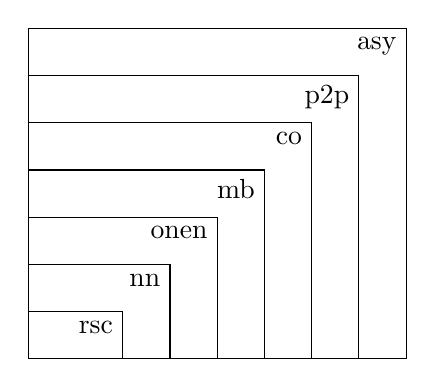
\begin{tikzpicture}[scale=0.6]
  % list of labels in order (from smallest to largest)
%   \def\labels{{rsc,nn,onen,mb,co,p2p,asy}}
  % loop to draw nested squares
  \foreach [count=\i] \lab in {rsc,nn,onen,mb,co,p2p,asy} {
    \draw (0,0) rectangle (\i+1,\i);
    \node[anchor=north east] at (\i+1,\i) {\lab};
  }
\end{tikzpicture}
\caption{Hierarchy of communication model semantics.}
\label{fig:coms}
\end{figure}

% A p2p-MSC is an MSC $M = (E,\to, \lhd, \lambda)$ where, for any two send events $s$ 
% and $s'$ such that $\lambda(s) \in \text{send}(p, q, \_), \lambda(s') in \text{send}(p, q, \_)$, 
% and $s \to^+ s'$, one of the following holds:
% - either $s, s' \in \text{matched}(M)$ with $s \lhd r$ and $s' \lhd r'$ and 
% $r \to^+ r'$,
% - or $s' \in \text{unmatched}(M)$.
% Note that we cannot have two messages $m 1$ and $m 2$, both sent by $p$ to $q$, 
% in that order, such that $m 1$ is unmatched and $m 2$ is matched; unmatched 
% message $m 1$ excludes the reception of any later message.

\paragraph{Causally ordered}
In the causally ordered (\verb|co|) communication model, messages are delivered 
to a process in accordance with the causal dependencies of their emissions. 
In other words, if there are two messages $m_1$ and $m_2$ with the same recipient, 
such that there exists a causal path from $m_1$ to $m_2$, then $m_1$ must be received 
before $m_2$. This notion of causal ordering was first introduced by Lamport under the 
name ``happened-before'' relation. In Figure~\ref{fig:p2p}, this 
causality is violated: $m_1$ should be received before $m_3$. Causal delivery 
is commonly implemented using Lamport's logical clock algorithm \cite{lamport2019time}.

% An MSC $M = (E, \to, \lhd, \lambda)$ is causally ordered if, for any two send $s$ and 
% $s'$, such that $\lambda(s) \in \text{send}(\_, q, \_), \lambda(s') \in \text{send}(\_, q, \_)$, and 
% $s \leq_{\text{hb}} s'$:
% - either $s, s' \in \text{matched}(M)$ and $r \to^* r'$, with $r$ and $r'$ receive 
% events such that $s \lhd r$ and $s' \lhd r'$.
% - or $s' \in \text{unmatched}(M)$.

% Note that in a \verb|co|-MSC we cannot have two send events $s$ and $s'$ addressed 
% to the same process, such that $s$ is unmatched, $s'$ is matched, and 
% $s \leq_{\text{hb}} s'$.

\paragraph{Mailbox}
In this model, any two messages sent to the same process, regardless of the sender, 
must be received in the same order as they are sent. If a process receives $m_1$ 
before $m_2$, then $m_1$ must have been sent before $m_2$. \verb|mb| coordinates all 
the senders of a single receiver. This model is also called FIFO $n-1$.
In Figure~\ref{fig:mailbox}, an example for this communication model is shown.

\begin{figure}[!ht]
	\centering
	\begin{msc}[draw frame=none, draw head=none, msc keyword=, 
				head height=0px, label distance=0.5ex, 
				foot height=0px, foot distance=0px]{}
		\declinst{p}{p}{}
		\declinst{q}{q}{}
		\declinst{r}{r}{}
		\declinst{s}{s}{}

		\mess[pos=0.1]{$m_4$}{p}{s}[4]
		\nextlevel
		\mess[pos=0.8]{$m_1$}{p}{q}
		\nextlevel
		\mess[pos=0.2]{$m_2$}{r}{q}
		\nextlevel
		\mess[pos=0.8]{$m_3$}{r}{s}
	\end{msc}
	\caption{An example of mailbox semantic.}
	\label{fig:mailbox}
\end{figure}

% An MSC $M = (E, \to, \lhd, \lambda)$ is a \verb|mb|-MSC if it has a linearization 
% $\rightsquigarrow$ where, for any two send events $s$ and $s'$, such 
% that $\lambda (s) \in \text{send}(\_,q,\_), \lambda (s') \in \text{send}(\_,q,\_)$, and 
% $s \rightsquigarrow s'$
% - either $s,s' \in \text{matched}(M)$ and $r \rightsquigarrow r'$, where 
% $s \lhd r$ and $s' \lhd r'$,
% - or $s' \in \text{unmatched}(M)$.

%% TODO: Esistono nella pratica? forse si possono togliere?

\paragraph{FIFO 1-n}
This model (\verb|onen|) is the dual of \verb|mb|, it coordinates a sender with all the 
receivers. Any two messages sent by a process must be received in the same 
order as they are sent. These two messages might be received by different 
processes and the two receive events might be concurrent.

% An MSC $M = (E, \to, \lhd, \lambda)$ is a \verb|onen|-MSC if it has a linearization 
% $\rightsquigarrow$ where, for any two send events $s$ and $s'$, such 
% that $\lambda (s) \in \text{send}(p,\_,\_), \lambda (s') \in \text{send}(p,\_,\_)$ and 
% $s \to^+ s'$ (which implies $s \rightsquigarrow s'$)
% - either $s,s' \in \text{matched}(M)$ and $r \rightsquigarrow r'$, with 
% $r$ and $r'$ receive events such that $s \lhd r$ and $s' \lhd r'$,
% - or $s' \in \text{unmatched}(M)$.

\paragraph{FIFO n-n}
In this model (\verb|nn|), messages are globally ordered and delivered according to 
their emission order. Any two messages must be received in the same order 
as they are sent. These two messages might be sent or receives by any process 
and the two send or receive events might be concurrent. The FIFO \verb|n-n| 
coordinates all the senders with all the receivers.

% An MSC $M = (E, \to, \lhd, \lambda)$ is a \verb|nn|-MSC if it has a linearization 
% $\rightsquigarrow$ where, for any two send events $s$ and $s'$, such 
% that $s \rightsquigarrow s'$
% - either $s, s' \in \text{matched}(M)$ and $r \rightsquigarrow r'$, with $r$ 
% and $r'$ receive events such that $s \lhd r$ and $s' \lhd r'$,
% - or $s' \in \text{unmatched}(M)$.
\paragraph{RSC}
Figure~\ref{fig:coms} shows \verb|rsc| as the last block of the hierarchy.
\verb|rsc| stands for \emph{Realisable in Synchronous Communication}, therefore, 
is comparable to our definition of $\synchmodel$ model, but there are 
some differences. For example, it does not accept \emph{orphan messages}, 
which are instead accepted for the definition of this thesis.

% \subsection{Realisability for Di Giusto et~al.}
% For the general model, we now recall the definition of 
% realisability. Recall that safe realisability correspond to weak 
% realisability with the addition of the deadlock freedom property.

% \bigskip

% \begin{definition}[Deadlock-free realisability]\label{def:realisability}
%     A global type $\gt$ is \emph{deadlock-free realisable}
%     in the communication model
%     $\acommunicationmodel$
%     if there is a system $\cfsms$ such that the following two conditions hold:
%     \begin{enumerate}
%     \item $\executionsof{\cfsms}{\acommunicationmodel} = 
%                 \executionsof{\gt}{\acommunicationmodel}$
%     \item $\cfsms$ is deadlock-free in $\acommunicationmodel$.
%     \end{enumerate}
% \end{definition}

% The first condition of Definition~\ref{def:realisability} corresponds to  
% the property of \emph{global type conformance}: all system executions 
% faithfully follow the behaviours prescribed by the global type.
% When $\acommunicationmodel$ is $\ppmodel$ or $\synchmodel$, 
% deadlock-free realisability coincides with the notion of 
% \emph{safe realisability} introduced in~\cite{alur2005realizability}.
% This equivalence does not extend to more general communication models, 
% such as the mailbox model, where 
% Proposition~\ref{prop:deadlock-free-as-a-property-on-mscs-for-p2p-and-synch} 
% fails to apply. Nonetheless, even in such settings, global type 
% conformance can still be expressed in terms of MSCs.


\section{Realisability for Alur and Lohrey}
We recall the definition of Safe Realisability for 
Alur~et~al.~\cite{alur2005realizability}.


We now introduce the definition of implementability following the one given 
by Alur, et al. \cite{alur2005realizability}, referred to as 
\textit{Weak-realisability}.
To formalize it, we first define the notions of 
\textit{weak implication} and \textit{weak closure}.

%% TODO: Spiegare meglio con intuizioni

\bigskip

\begin{definition}[Weakly-imply]
	Let $\setmsc$ be a set of MSCs and $M$ an MSC. $\setmsc$
	\textit{weakly implies} $M$, if for any sequence of automata
	$\langle A_i \ |\ 1\leq i\leq n\rangle$, if every MSC in $\setmsc$ is in
	$L(\prod_i A_i)$ then $M \in L(\prod_i A_i)$.
\end{definition}

In order to understand the meaning of \emph{weak implication},
consider the following example.

\bigskip

\begin{example}
Define two MSCs, MSC1 and MSC2. Both perform the same four
communications, but in different orders.  
MSC1 first sends message $a$ from P1 to P2, then from P1 to P3, 
then sends $b$ from P4 to P2, and finally from P4 to P3.  
MSC2 instead starts with P4 sending $b$ to P2, then to P3, 
followed by P1 sending $a$ to P2 and then to P3.  

Now define a third MSC $M$ with the same four messages but in a
different order: P1 sends $a$ to P2, P4 sends $b$ to P2, P4 sends 
$b$ to P3, and finally P1 sends $a$ to P3.  

We say $M$ is weakly implied by MSC1 and MSC2. Indeed, by looking
at each process projection we recover the same behaviour in one of
them: for P1 and P4 in both, for P2 in MSC1, and for P3 in MSC2.  
Figure~\ref{fig:weak-impl} illustrates the three MSCs.

\begin{figure}[!ht]
\centering
\begin{tabular}{ccc}
\begin{minipage}{0.32\textwidth}
\scalebox{0.55}{%
\begin{msc}[left environment distance=0cm, draw frame=none, draw head=none, msc keyword=, head height=0px, label distance=0.5ex, foot height=0px, foot distance=0px]{}
	\declinst{P1}{P1}{}
	\declinst{P2}{P2}{}
	\declinst{P3}{P3}{}
	\declinst{P4}{P4}{}

	\mess{a}{P1}{P2}
	\nextlevel
	\mess[pos=0.25]{a}{P1}{P3}
	\nextlevel
	\nextlevel
	\mess[pos=0.25]{b}{P4}{P2}
	\nextlevel
	\mess{b}{P4}{P3}
\end{msc}
} 
\end{minipage}
&
\begin{minipage}{0.32\textwidth}
\scalebox{0.55}{%
\begin{msc}[left environment distance=0cm, draw frame=none, draw head=none, msc keyword=, head height=0px, label distance=0.5ex, foot height=0px, foot distance=0px]{}
	\declinst{P1}{P1}{}
	\declinst{P2}{P2}{}
	\declinst{P3}{P3}{}
	\declinst{P4}{P4}{}

	\mess[pos=0.25]{b}{P4}{P2}
	\nextlevel
	\mess{b}{P4}{P3}
	\nextlevel
	\nextlevel
	\mess{a}{P1}{P2}
	\nextlevel
	\mess[pos=0.25]{a}{P1}{P3}
\end{msc}
}
\end{minipage}
&
\begin{minipage}{0.32\textwidth}
\scalebox{0.55}{%
\begin{msc}[left environment distance=0cm, draw frame=none, draw head=none, msc keyword=, head height=0px, label distance=0.5ex, foot height=0px, foot distance=0px]{}
	\declinst{P1}{P1}{}
	\declinst{P2}{P2}{}
	\declinst{P3}{P3}{}
	\declinst{P4}{P4}{}

	\mess{a}{P1}{P2}
	\nextlevel
	\mess[pos=0.25]{b}{P4}{P2}
	\nextlevel
	\nextlevel
	\mess{b}{P4}{P3}
	\nextlevel
	\mess[pos=0.25]{a}{P1}{P3}
\end{msc}
}
\end{minipage} \\
MSC1 & MSC2 & $M$
\end{tabular}
\caption{The MSC $M$ is weakly implied by MSC1 and MSC2}
\label{fig:weak-impl}
\end{figure}
\end{example}

\bigskip

\begin{definition}[Weakly-closure $\setmsc^w$]
	The weak-closure $\setmsc^w$ of a set $\setmsc$ of MSCs contains all the MSCs
	weakly implied by $\setmsc$.
\end{definition}

% todo: esempio

\bigskip

\begin{definition}[Weakly-realisable]\label{def:weak-realisability}
	An MSC $M$ is said to be weakly-realisable if the set of MSCs
	$L(M)$ is weakly realisable. A set of MSCs $\setmsc$ is said to be weakly
	realisable if $\setmsc=\setmsc^w$.
\end{definition}
It is important to note that this definition does not include the
property of deadlock-freedom. 

\bigskip

\begin{definition}[Safe Realisability~\cite{alur2005realizability}]
Let $L$ be a set of MSCs. Then $L$ is said to be \emph{safely realisable}
if there exists a family of concurrent automata 
$\langle A_i \mid 1 \leq i \leq n \rangle$ such that
$ L = L(\prod_i A_i)$ and 
$\prod_i A_i$ is deadlock-free.

Equivalently, $L$ is safely realisable iff it satisfies the following two
closure conditions, where $\mathit{pref}(L)$ denotes the set of prefixes 
of the MSCs (or words) in $L$:
\begin{enumerate}
  \item For every well-formed word $w$ (a partial MSC), if for all 
  $1 \leq i \leq n$ there exists a word $v_i \in \mathit{pref}(L)$ 
  such that $w{\upharpoonright_i} = v_i{\upharpoonright_i}$, then 
  $w \in \mathit{pref}(L)$.
  \item For every well-formed and complete word $w$ (an MSC) in 
  $\mathit{pref}(L)$, if for all $1 \leq i \leq n$ there exists a 
  word $v_i \in L$ such that $w{\upharpoonright_i} = v_i{\upharpoonright_i}$, 
  then $w \in L$.
\end{enumerate}
\end{definition}


For finite sets of MSCs, weakly realisability as defined in 
\cite{alur2005realizability}, as defined in this thesis 
(Definition~\ref{def:weak-realisability}), is \verb|coNP|-complete and safe 
realisability is shown to be decidable in \verb|P|-time~\cite{alur2005realizability}.
The problem was subsequently studied for HMSCs. For bounded HMSCs, safe realisability 
remains decidable, but weak realisability 
is undecidable~\cite{alur2005realizability}. Extensions of these results to non-FIFO 
semantics were investigated in~\cite{morin2002recognizable}, corresponding 
to bag semantics under peer-to-peer communication. 
Later, Lohrey proved, with a technique that involves five processes, 
that in the general case, safe realisability 
is undecidable~\cite{lohrey2003realizability}, though it is decidable (and 
\verb|EXPSPACE|-complete) for globally cooperative HMSCs. % TODO: capire cos'è globally cooperative
Most positive results assume bounded channels, but \cite{bollig2025high} introduces 
a new class of HMSCs that allows unbounded channels while maintaining implementability.
A summary of the main complexity results is given in Table~\ref{tab:realisability}.

\begin{table}[!ht]
	\centering
	\begin{tabular}{|l|c|c|c|}
		\hline
		& \textbf{Finite set} & \textbf{Bounded graphs} & \textbf{Unbounded} \\
		\hline
		\textbf{Weak} & \verb|coNp|-complete & undecidable & undecidable \\
		\hline
		\textbf{Safe} & P-time & \verb|EXPSPACE|-complete & undecidable \\
		\hline
	\end{tabular}
	\caption{Summary of results on realisability.}
	\label{tab:realisability}
\end{table}

\section{Realisability for MPST}

Recent work has focused on addressing the connection between MPST 
and automata-theoretic formalisms. Stutz and Zufferey 
showed that implementability is decidable by encoding global types 
into HMSCs that are globally cooperative~\cite{stutz2022comparing,stutz2023asynchronous}. 
Building on this, Li et al.~\cite{li2023complete} proposed a complete 
projection function for MPST, guaranteeing that every implementable 
global type admits a correct distributed implementation.

Stutz’s thesis~\cite{stutz2024implementability} connects MPST to 
High-level MSCs (HMSCs), introducing a generalized projection operator 
for sender-driven choice where a sender may branch towards different 
receivers. This captures patterns beyond classical MPST projection.  
He also proves that while syntactic projection is incomplete, 
an automata-theoretic encoding into HMSCs yields decidability for 
sender-driven choice, with implementability shown to be in 
\verb|PSPACE|-the first precise complexity bound for this fragment.

We recall the definition of the \emph{Implementability Problem} as 
introduced by Stutz et al.~\cite{stutz2024implementability}.  

\bigskip

\begin{definition}[Implementability Problem~\cite{stutz2024implementability}]
A language $L \subseteq \Gamma^\omega$ is said to be 
\emph{implementable} if there exists a CSM 
$\{A_p\}_{p \in \mathbb{P}}$ such that
\begin{itemize}
    \item \textbf{deadlock freedom:} 
    $\{A_p\}_{p \in \mathbb{P}}$ is deadlock-free, and
    \item \textbf{protocol fidelity:} 
    $L$ is the language of $\{A_p\}_{p \in \mathbb{P}}$.
\end{itemize}
\end{definition}

where the definition of deadlock freedom is:

\bigskip

\begin{definition}[Deadlock freedom~\cite{stutz2024implementability}]
A configuration for an automaton is a deadlock if it is not final and  
has no outgoing transitions while it is reachable if it occurs on some 
run of A. A CSM is deadlock-free if no reachable configuration is a
deadlock. We say a CSM is sink-final if all its state machines are.
\end{definition}

\section{Choreographies}
Choreographies \cite{montesi2014choreographic} are another formalism to describe  
distributed communication protocols. Unlike MSCs or MPST, which focus either on 
trace-based semantics or type systems, choreographies emphasize the 
global specification of interactions as a high-level description of the 
intended message exchanges. Similarly to MPST, their goal is to ensure that
a distributed  implementation can be derived in which each participant 
follows a local behaviour consistent with the global description, called
respectively \emph{local} and \emph{global-view}. This setting naturally 
connects to the realisability problem, since the key question is whether 
a choreography can be faithfully implemented by a system of local 
processes. In choreographies, the local-view is called \textbf{End-Point Projection} (EPP),
and it is derived throughout a projection operation from the global-view.
The \emph{knowledge of choice} problem is similar to the implementability one,
and explored also in choreographies,
but it was first introduced by Castagna et al.~\cite{castagna2012global}.
% https://www.fabriziomontesi.com/bliki/KnowledgeOfChoice#CHY12
% TODO: Continuare menzionando che i chor automata sono simili alla nostra 
% definizione di global type

\section{Multiparty Session Types}
Multiparty Session Types (MPST)~\cite{honda2008multiparty} 
provide a type-theoretic framework to specify and verify communication 
protocols among multiple participants. They ensure that communication 
follows a predefined structure, preventing errors such as deadlocks, 
orphan messages, and unspecified receptions. The 
\textbf{global specification} describes the overall communication 
protocol. From this, one derives the \textbf{local behaviours} of each 
participant via a \emph{projection} operation. The system's 
\textbf{processes} form the \emph{implementation}, defining how 
participants interact. With the definition of a \emph{typing system} 
and suitable \emph{type-checking rules}, one ensures that the 
implementation conforms to the local specification, thereby 
guaranteeing properties such as \emph{well-formedness}.  
Figure~\ref{fig:mpstschema} show a schema summarizing the principal
parts of the framework.

\begin{figure}[!ht]
\centering
\begin{tikzpicture}[
      node distance=1.2cm,
      every node/.style={font=\sffamily},
      rect/.style={rectangle, draw=black, minimum width=1cm, minimum height=1cm},
      circ/.style={circle, draw=black, minimum size=1cm},
      arrow/.style={-{Stealth[scale=1.1]}, thick}
  ]

  % Nodes
  \node[rect] (G) {\textcolor{red}{$\mathcal{G}$}};
  \node[circ, below=of G] (TB) {\textcolor{blue}{$L_\text{B}$}};
  \node[circ, left=of TB] (TA) {\textcolor{blue}{$L_\text{A}$}};
  \node[circ, right=of TB] (TC) {\textcolor{blue}{$L_\text{C}$}};

  \node[rect, below=of TA] (PA) {\textcolor{brown}{$P_\text{A}$}};
  \node[rect, below=of TB] (PB) {\textcolor{brown}{$P_\text{B}$}};
  \node[rect, below=of TC] (PC) {\textcolor{brown}{$P_\text{C}$}};

  \node[rect,draw=none,right=of TC] (LC) {\textbf{\textcolor{blue}{2. Local type}}};
  \node[rect,draw=none,above=of LC] (LG) {\textbf{\textcolor{red}{1. Global type}}};
  \node[rect,draw=none,below=of LC] (LG) {\textbf{\textcolor{brown}{3. Processes}}};

  % Arrows
  \draw[arrow] (G) -- (TA) node[midway, left] {Projection};
  \draw[arrow] (G) -- (TB);
  \draw[arrow] (G) -- (TC);

  \draw[arrow] (PA) -- (TA) node[midway, left] {Type checking};
  \draw[arrow] (PB) -- (TB);
  \draw[arrow] (PC) -- (TC);
  \draw[arrow] (TC) -- (PC);
  \draw[arrow] (TB) -- (PB);
  \draw[arrow] (TA) -- (PA);

\end{tikzpicture}
\caption{Intuitive schema of MPST framework}
\label{fig:mpstschema}
\end{figure}

% In this setting, the analogue of realisability is often called 
% \emph{session fidelity}: a property ensuring that the combined local 
% types behave exactly according to the global type. When the global 
% type satisfies syntactic restrictions, its projection is guaranteed 
% to be both realisable and deadlock-free, which corresponds to safe 
% realisability in the MSC setting.  

\subsection{Projectability}
A central notion in MPST is \emph{projectability}, which asks whether 
a global type can be faithfully projected into local specifications for 
each participant. If projection succeeds, the resulting local types 
interact without mismatches or unintended behaviours, effectively 
bridging global specifications and distributed implementations~\cite{honda2008multiparty}.  
Projectability is, therefore, comparable to the implementability
problem as they have the same aim.
Projection algorithms, however, often reject natural protocols that 
fail to meet restrictive syntactic conditions. This difference between 
expressivity and safety has motivated extensions of the theory, with 
\cite{castagna2012global} being the only algorithm aiming for full 
completeness.

% \subsubsection{Mixed and Sender driven choice}
A key restriction in the definition of MPST appears in branching. 
In the original framework \cite{honda2008multiparty,carbone2012structured}, 
choice is \textbf{sender-driven}: the first sender dictates the branch, 
ensuring safety but excluding many common patterns where multiple 
participants influence the decision~\cite{carbone2012structured}.  
Allowing \textbf{mixed choice} increases expressivity by permitting 
several initiators, but it also makes the implementability problem 
undecidable in general~\cite{stutz2024implementability}.  

\section{Other works}
%citare il paper di Emilio su pomsets
Stutz et al.~\cite{stutz2025automata} proposed \emph{Protocol State Machines} 
(PSMs), an automata-based formalism subsuming both MPST and HMSCs. 
PSMs show that many syntactic restrictions of global types are not 
true expressivity limits. Yet, the implementability problem for PSMs 
with unrestricted mixed choice remains undecidable, resolving the 
open question that mixed-choice global types are undecidable in general.  

In summary, projectability is well understood for sender-driven choice, 
where decidability and complexity bounds are established, but moving 
towards mixed choice inevitably leads to undecidability. Automata-based 
techniques such as HMSCs and PSMs provide the most powerful tools for 
extending the theory while preserving decidability in restricted cases.